\chapter{THIẾT KẾ Ổ LĂN}
    \section{THIẾT KẾ Ổ TRÊN TRỤC II}
        \subsection{Phân tích lực tác dụng lên ổ}
            \begin{figure}[H]
                \centering
                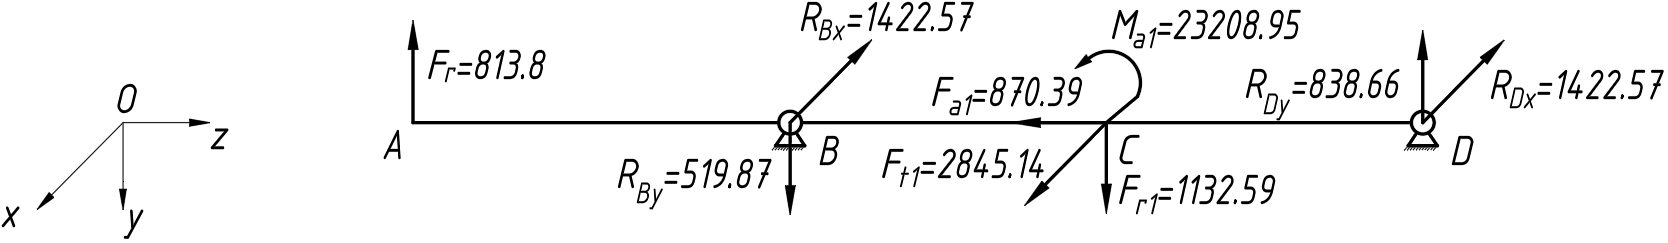
\includegraphics[width=1\textwidth]{pictures/bearing_II.png}
                \caption{Lực tác dụng lên ổ trục II}
            \end{figure}
            \subsubsection{Xác định phản lực tác dụng lên ổ}
                \[
                    F_{r} = \sqrt{F_{rx}^2 + F_{ry}^2} = \sqrt{R_{x}^2 + R_{y}^2}\footnote{Trích tài liệu \cite{gtctm}, trang 442, công thức 11.17}
                \]
                \begin{itemize}
                    \item Phản lực tác dụng lên ổ B:
                        \begin{align*}
                            F_{rB} &= \sqrt{R_{Bx}^2 + R_{By}^2} = \sqrt{1314.8^2 + 586.21^2} = 1439.56\, \mathrm{N}
                        \end{align*}
                    \item Phản lực tác dụng lên ổ D:
                        \begin{align*}
                            F_{rD} &= \sqrt{R_{Dx}^2 + R_{Dy}^2} = \sqrt{1530.34^2 + 905^2} = 1777.91\, \mathrm{N}
                        \end{align*}
                \end{itemize}
                \hspace*{0.6cm}Vì $F_{rB} < F_{rD}$ nên ta sẽ tính toán chọn ổ lăn theo ổ lăn D. $F_{r} = F_{rD} = 1777.91\, \mathrm{N}$
            \subsubsection{Xác định lực dọc trục tác dụng lên ổ}
                \begin{align*}
                    F_{a} = F_{a1} = 870.39\, \mathrm{N}
                \end{align*}
        \subsection{Chọn sơ bộ ổ lăn}
            \begin{figure}[H]
                \centering
                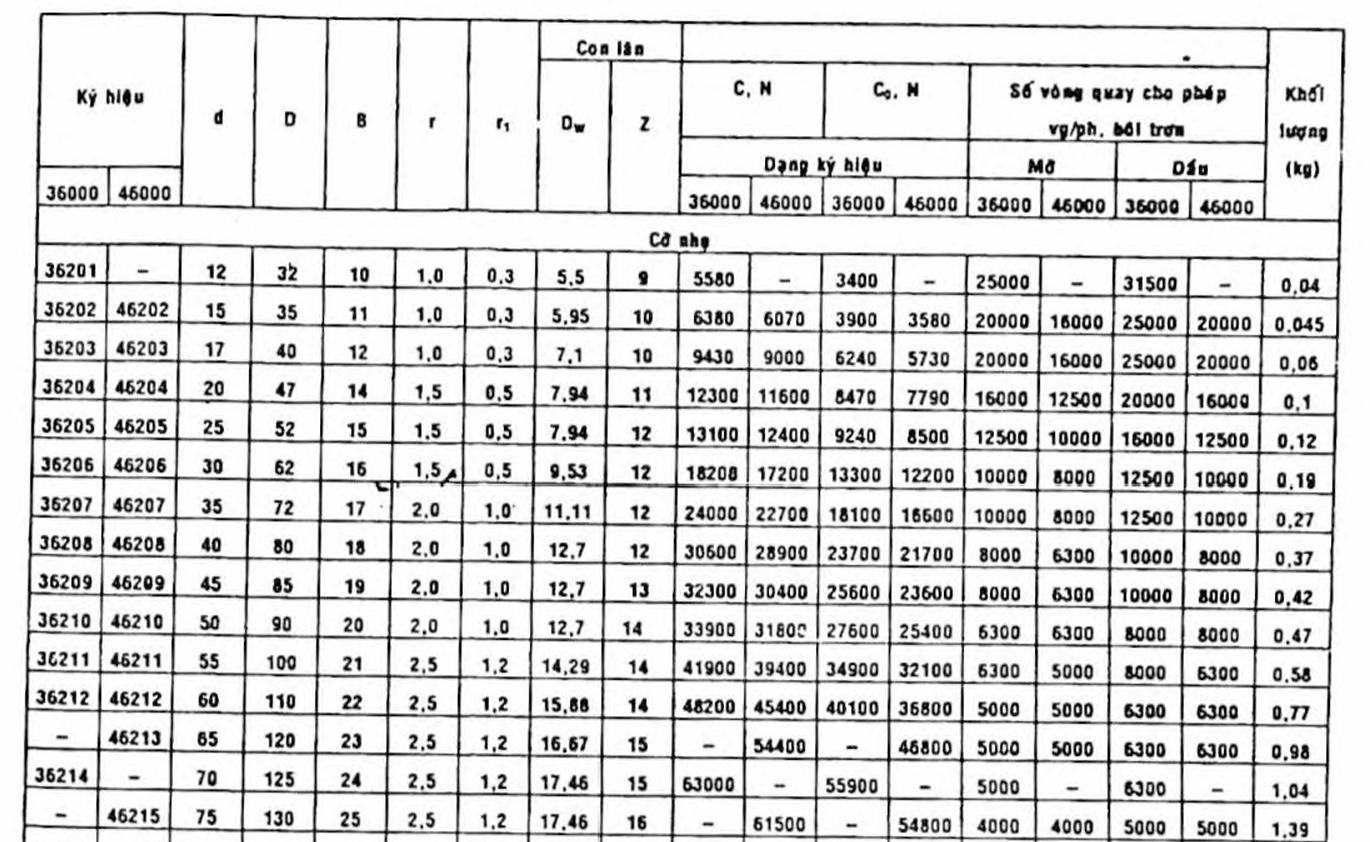
\includegraphics[width=1\textwidth]{pictures/bearing_standard_II.png}
                \caption{Tiêu chuẩn ổ đỡ chặn}
                \caption*{\footnotesize(Trích tài liệu \cite{btctm}, trang 512, phụ lục 9.3)}
            \end{figure}
            \begin{itemize}
                \item Ta có: $0.3 \leq \frac{F_a}{F_r} = \frac{870.39}{1777.91} = 0.489 \leq 0.7$. \\[0.3cm]
                    $\Rightarrow$ Chọn loại ổ là ổ bi đỡ chặn 1 dãy.
                \item Ta có đường kính trục tại ổ lăn: $d = d_{B} = d_{D} = 30\, \mathrm{mm}$
                \item Chọn ổ lăn là ổ bi đỡ chặn, cỡ nhẹ có ký hiệu 36206  $(\alpha = 12 ^\circ)$ với $C = 18208\, \mathrm{N}$ và $C_o = 13300\, \mathrm{N}$.
                \item Chọn cấp chính xác cho ổ lăn là 0. Có độ đảo hướng tâm $20\, \mathrm{\mu m}$. Giá thành tương đối là 1.
            \end{itemize}
        \subsection{Tính ổ lăn theo khả năng tải động}
            \subsubsection{Chọn các hệ số}
                \begin{itemize}
                    \item Chọn hệ số $K_{\sigma} = 1$ do tải trọng tỉnh.
                    \item Chọn hệ số $K_{t} = 1$ do làm việc ở nhiệt độ bình thường.
                    \item Chọn hệ số $V = 1$ do vòng trong quay.
                    \item Chọn hệ số X và Y:
                        \begin{itemize}
                            \item Tỉ số $\frac{F_{a}}{C_{o}} = \frac{870.39}{13300} = 0.065 \Rightarrow$ Chọn $e = 0.38$.
                            \item Tỉ số $\frac{F_{a}}{VF_{r}} = \frac{870.39}{1 \cdot 1777.91} = 0.49 > e \Rightarrow$ Chọn $X = 0.45$ và $Y = 1.45$.
                        \end{itemize}
                \end{itemize}
            \subsubsection{Tính khả năng tải động}
                \begin{itemize}
                    \item Thời gian làm việc tính bằng triệu vòng quay:
                        \[
                            L = \frac{60nL_{h}}{10^6}\footnote{Trích tài liệu \cite{gtctm}, trang 449, công thức 11.25b} = \frac{60 \cdot 360 \cdot 24000}{10^6} = 518.4\, \textrm{triệu vòng} 
                        \]
                    \item Tải trọng quy ước tác dụng lên ổ lăn:
                        \[
                            Q = Q_{r} = (XVF_{r} + YF_{a}) \cdot K_{\sigma}K_{t} \footnote{Trích tài liệu \cite{gtctm}, trang 444, công thức 11.20} = (0.45 \cdot 1 \cdot 1777.91 + 1.45 \cdot 870.39) \cdot 1 \cdot 1 = 2062.13\, \mathrm{N}
                        \]
                    \item Khả năng tải động tính toán của ổ:
                        \[
                            C_{tt} = Q \cdot \sqrt[m]{L} \footnote{Trích tài liệu \cite{gtctm}, trang 450, công thức 11.27} = 2062.13 \cdot \sqrt[3]{518.4} = 16565.49\, \mathrm{N}
                        \
                        \]
                        Ta có: $C_{tt} = 16065.49\, \mathrm{N} < C = 18208\, \mathrm{N}$ $\Rightarrow$ Thỏa điều kiện tải tĩnh.
                \end{itemize}
                \begin{table}[H]
                    \centering
                    \begin{tabular}{|c|c|c|c|c|c|c|c|c|c|}
                        \hline
                        \textbf{Ký hiệu} & \textbf{d, mm} & \textbf{D, mm} & \textbf{B, Nm} & \textbf{r, mm} & $\mathbf{r_{1}, mm}$ & $\mathbf{C, N}$ & $\mathbf{C_{o}, N}$ & $\mathbf{L_{h}}$, \textbf{giờ} \\
                        \hline
                        36206 & 30 & 62 & 16 & 1.5 & 0.5 & 18208 & 13300 & 24000 \\
                        \hline
                    \end{tabular}
                    \caption{Bảng số liệu về con lăn trục II}
                \end{table}
    \section{THIẾT KẾ Ổ TRÊN TRỤC III}
        \subsection{Phân tích lực tác dụng lên ổ}
            \begin{figure}[H]
                \centering
                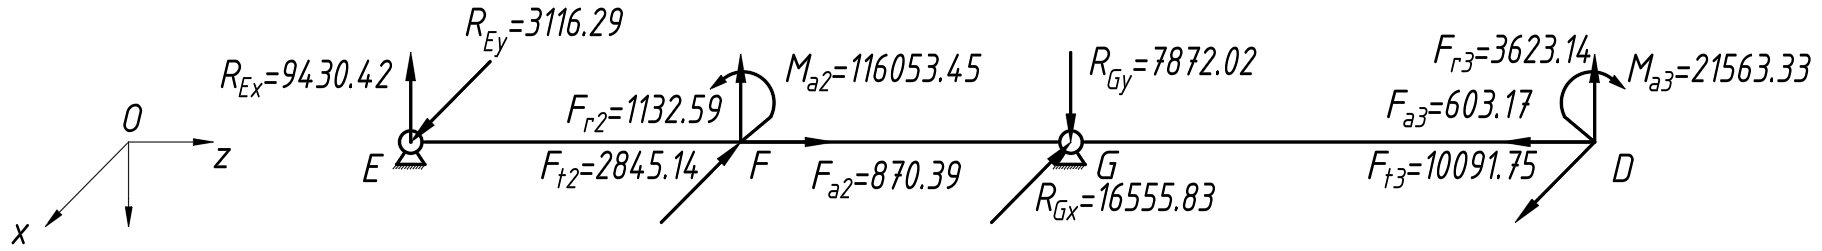
\includegraphics[width=1\textwidth]{pictures/bearing_III.png}
                \caption{Lực tác dụng lên ổ trục III}
            \end{figure}
            \subsubsection{Xác định phản lực tác dụng lên ổ}
                \[
                    F_{r} = \sqrt{F_{rx}^2 + F_{ry}^2} = \sqrt{R_{x}^2 + R_{y}^2}
                \]
                \begin{itemize}
                    \item Phản lực tác dụng lên ổ E:
                        \begin{align*}
                            F_{rE} &= \sqrt{R_{Ex}^2 + R_{Ey}^2} = \sqrt{9309.2^2 + 2924.38^2} = 9757.72\, \mathrm{N}
                        \end{align*}
                    \item Phản lực tác dụng lên ổ G:
                        \begin{align*}
                            F_{rG} &= \sqrt{R_{Gx}^2 + R_{Gy}^2} = \sqrt{16555.83^2 + 7680.11^2} = 18250.47\, \mathrm{N}
                        \end{align*}
                \end{itemize}
                \hspace*{0.6cm}Vì $F_{rE} < F_{rG}$ nên ta sẽ tính toán chọn ổ lăn theo ổ lăn G. $F_{r} = F_{rG} = 18250.47\, \mathrm{N}$
            \subsubsection{Xác định lực dọc trục tác dụng lên ổ}
                \begin{align*}
                    F_{a} = |F_{a2} - F_{a3}| = |870.39 - 603.17| = 267.22\, \mathrm{N}
                \end{align*}
        \subsection{Chọn sơ bộ ổ lăn}
            \begin{figure}[H]
                \centering
                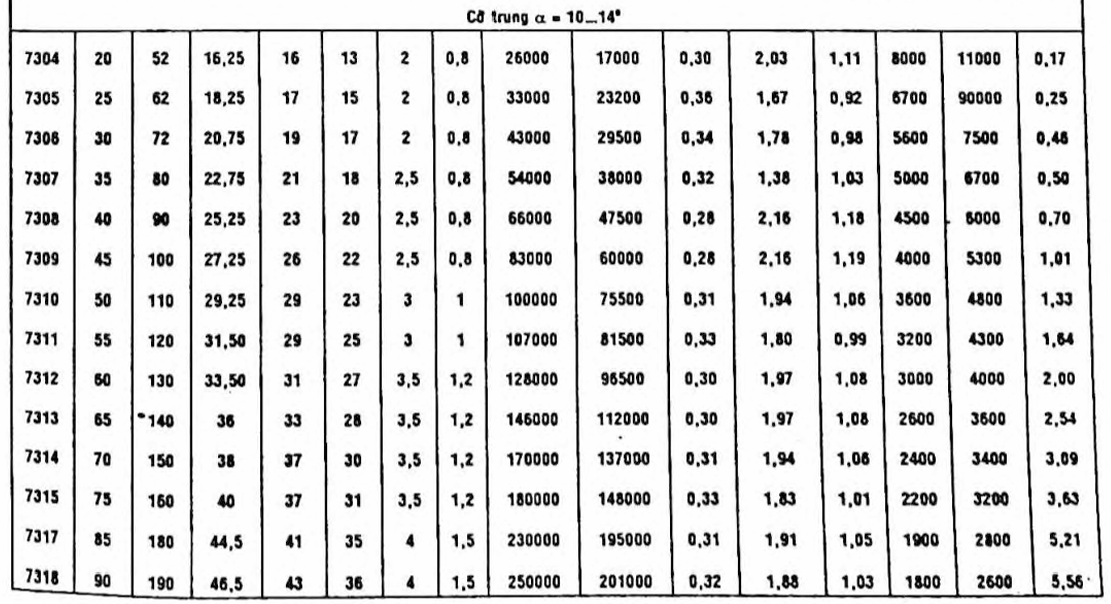
\includegraphics[width=1\textwidth]{pictures/bearing_standard_III.png}
                \caption{Tiêu chuẩn ổ đũa côn}
                \caption*{\footnotesize(Trích tài liệu \cite{btctm}, trang 512, phụ lục 9.3)}
            \end{figure}
            \begin{itemize}
                \item Ta có: $\frac{F_a}{F_r} = \frac{267.22}{18250.47} = 0.015 \leq 0.3$. \\[0.3cm]
                Để đảm bảo độ cứng ổ cao ta chọn loại ổ là ổ đũa côn.
                \item Ta có đường kính trục tại ổ lăn: $d = d_{E} = d_{G} = 50\, \mathrm{mm}$
                \item Chọn ổ lăn là ổ đũa côn, cỡ trung có ký hiệu 7310 với $C = 100000\, \mathrm{N}$ và $C_o = 75500\, \mathrm{N}$.
                \item Chọn cấp chính xác cho ổ lăn là 0. Có độ đảo hướng tâm $20\, \mathrm{\mu m}$. Giá thành tương đối là 1.
            \end{itemize}
        \subsection{Tính ổ lăn theo khả năng tải động}
            \subsubsection{Chọn các hệ số}
                \begin{itemize}
                    \item Chọn hệ số $K_{\sigma} = 1$ do tải trọng tỉnh.
                    \item Chọn hệ số $K_{t} = 1$ do làm việc ở nhiệt độ bình thường.
                    \item Chọn hệ số $V = 1$ do vòng trong quay.
                    \item Chọn hệ số X và Y:
                        \begin{itemize}
                            \item Tỉ số $\frac{F_{a}}{C_{o}} = \frac{267.22}{75500} = 0.003 \Rightarrow$ Chọn $e = 0.3$.
                            \item Tỉ số $\frac{F_{a}}{VF_{r}} = \frac{267.22}{1 \cdot 18250.47} = 0.015 < e \Rightarrow$ Chọn $X = 1$ và $Y = 0$.
                        \end{itemize}
                \end{itemize}
            \subsubsection{Tính khả năng tải động}
                \begin{itemize}
                    \item Thời gian làm việc tính bằng triệu vòng quay:
                        \[
                            L = \frac{60nL_{h}}{10^6} = \frac{60 \cdot 72 \cdot 24000}{10^6} = 103.68\, \textrm{triệu vòng} 
                        \]
                    \item Tải trọng quy ước tác dụng lên ổ lăn:
                        \[
                            Q = Q_{r} = (XVF_{r} + YF_{a}) \cdot K_{\sigma}K_{t} = (1 \cdot 1 \cdot 18250.47 + 0 \cdot 267.22) \cdot 1 \cdot 1 = 18250.47\, \mathrm{N}
                        \]
                    \item Khả năng tải động tính toán của ổ:
                        \[
                            C_{tt} = Q \cdot \sqrt[m]{L} = 18250.47 \cdot \sqrt[3]{103.68} = 85737 \, \mathrm{N}
                        \]
                        Ta có:  $C_{tt} = 85737\, \mathrm{N} < C = 100000\, \mathrm{N}$ $\Rightarrow$ Thỏa điều kiện tải tĩnh. 
                \end{itemize} 
                \begin{table}[H]
                    \centering
                    \begin{tabular}{|c|c|c|c|c|c|c|c|c|}
                        \hline
                        \textbf{Ký hiệu} & \textbf{d, mm} & \textbf{D, mm} & \textbf{B, Nm} & \textbf{r, mm} & $\mathbf{C, N}$ & $\mathbf{C_{o}, N}$ & $\mathbf{L_{h}}$, \textbf{giờ} \\
                        \hline
                        7310 & 50 & 110 & 29 & 3 & 100000 & 75500 & 24000 \\
                        \hline
                    \end{tabular}
                    \caption{Bảng số liệu về con lăn trục III}
                \end{table}

                    
                
            